\chapter{Response Manager}
\label{chap_state}

Response Manager utamanya berfungsi untuk menghasilkan Status Word (SW) yang sesuai dengan Response Type dari Command Handler, untuk kemudian dikirimkan oleh Transmission Handler SendSW. Table \ref{tabel-swlist} menampilkan daftar Response Type dan Status Word yang sesuai.

\begin{table}[h]
  \centering
  \begin{tabular}{|c|c|}
    \hline
    Response Type & Status Word \\
    \hline
    OK & 9000 \\
    Normal & 6100 \\
    Counter & 63C0 \\
    Wrong Length & 6700 \\
    Not Supported & 6800 \\
    Not Allowed & 6900 \\
    Security Status & 6982 \\
    Auth Blocked & 6983 \\
    Condition Not Satisfied & 6985 \\
    Wrong P1P2 & 6A00 \\
    File Not Found & 6A82 \\
    INS Not Supported & 6D00 \\
    CLA Not Supported & 6E00 \\
    Fatal Error & 6F00 \\
    \hline
  \end{tabular}
  \caption{Daftar Response Type dan Status Word yang sesuai}
  \label{tabel-swlist}
\end{table}

Response Type sendiri dideklarasikan sebagai sebuah tipe data enumerasi sebagaimana ditunjukkan pada Listing \ref{list-rspntype}, dan dapat ditemukan pada file header $response.h$.

\begin{lstlisting}[caption={Tipe Data Enumerasi Response Type}, label={list-rspntype}]
typedef enum
{
  Response_OK,
  Response_Normal,
  Response_Counter,
  Response_WrongLength,
  Response_NotSupported,
  Response_CmdNotAllowed,
  Response_AuthBlocked,
  Response_ConditionNotSatisfied,
  Response_WrongP1P2,
  Response_FileNotFound,
  Response_INSNotSupported,
  Response_CLANotSupported,
  Response_FatalError,
} rspn_type;
\end{lstlisting}

Beberapa Response Type dapat menerima parameter tambahan untuk menjelaskan response secara lebih terperinci. Sebagai contoh response type Normal dapat memuat parameter tambahan untuk menunjukkan jumlah byte yang masih tersedia sebagai response data untuk dapat diambil selanjutnya menggunakan command Get Response oleh Terminal. Response Type lainnya yang dapat menerima parameter tambahan ini adalah Counter, dengan parameter tambahan menunjukkan percobaan yang telah dilakukan dan gagal ketika melakukan verifikasi PIN. Status Word yang dihasilkan untuk response type dengan parameter tambahan ini adalah:

\begin{equation}
status\_word \mathrel{|} extra\_parameter
\end{equation}

Sebagai contoh untuk response type Counter ($63C0$) dengan parameter tambahan $2$ (yang berarti telah gagal melakukan verifikasi sebanyak 2 kali), akan menghasilkan response type $63C2$.

Status Word ini kemudian akan disimpan dalam sebuah variabel unsigned integer 16 bit sebagai ditunjukkan pada Listing \ref{list-statusword}, dan dapat ditemukan pada file header $response.h$.

\begin{lstlisting}[caption={Deklarasi variabel status word}, label={list-statusword}]
uint16_t sw;
\end{lstlisting}

\section{Response Set SW}
\label{sec_setsw}

Berfungsi memetakan response type dengan Status Word (SW) yang sesuai. Gambar \ref{fig-dfd-setsw} menampilkan DFD dari fungsi Response Set SW. Diagram alir fungsi kemudian ditampilkan pada Gambar \ref{fig-flow-setsw}. 

\begin{figure}[h]
\centering
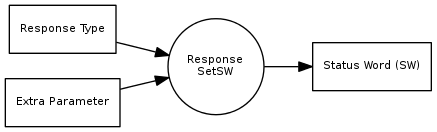
\includegraphics[scale=0.75]{image/response/dfd_setsw.png}
\caption{DFD Response Set SW}
\label{fig-dfd-setsw}
\end{figure}

\begin{figure}[h]
\centering
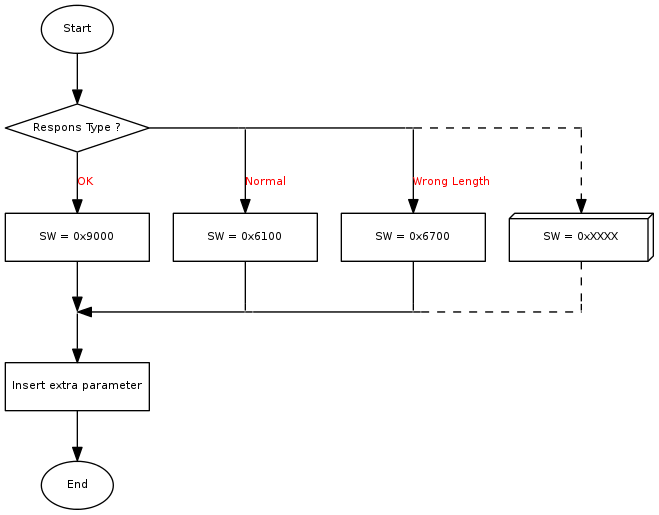
\includegraphics[scale=0.5]{image/response/flow_setsw.png}
\caption{Flowchart Response Set SW}
\label{fig-flow-setsw}
\end{figure}

\subsection {Pengujian}

\begin{table}[h]
  \centering
  \begin{tabular}{ | c | c || c | }
    \hline
    \multicolumn{2}{ |c|| }{Input}  & Output \\
    \hline
    response type & extra parameter & status word\\
    \hline
    OK & 0 & = 9000 \\
    Normal & 0 & = 6100 \\
    Counter & 0 & = 63C0 \\
    Wrong Length & 0 & = 6700 \\
    Not Supported & 0 & = 6800 \\
    Not Allowed & 0 & = 6900 \\
    Security Status & 0 & = 6982 \\
    Auth Blocked & 0 & = 6983 \\
    Condition Not Satisfied & 0 & = 6985 \\
    Wrong P1P2 & 0 & = 6A00 \\
    File Not Found & 0 & = 6A82 \\
    INS Not Supported & 0 & = 6D00 \\
    CLA Not Supported & 0 & = 6E00 \\
    Fatal Error & 0 & = 6F00 \\
    Normal & 0F & = 610F \\
    Counter & 03 & = 63C3 \\
    \hline
  \end{tabular}
  \caption{Test Vector Fungsi Response Set SW}
  \label{tabel-test-setsw}
\end{table}

Tabel \ref{tabel-test-setsw} menampilkan Test Vector yang digunakan untuk menguji fungsi Response Set SW.


\subsection {Implementasi}

Tabel \ref{tabel-setsw} menampilkan purwarupa dari implementasi fungsi Set SW. 

\begin{table}[h]
  \centering
  \begin{tabular}{m{2cm} p{8cm}}
    \hline
    {\bf Name} & Response\_SetSW\\
    \hline
    {\bf Input} & 
    \begin{itemize}[noitemsep,topsep=0pt,parsep=0pt,partopsep=0pt]
    \item response - Response Type (unsigned integer 8 bit)
    \item extra - Extra Parameter (unsigned integer 8 bit)
    \end{itemize}
    \\
    \hline
    {\bf Output} & None
    \\
    \hline
  \end{tabular}
  \caption{Prototype Fungsi Response Set SW}
  \label{tabel-setsw}
\end{table}

Listing \ref{list-setsw} menampilkan bagian program yang mengimplementasi fungsi Response Set SW, dan dapat ditemukan pada file $response.c$.

\begin{lstlisting}[caption={Implementasi Fungsi Response Set SW}, label={list-setsw}]
void Response_SetSW( rspn_type response, uint8_t extra )
{
  switch( response ) 
    {
    case Response_OK:
      sw = 0x9000;
    case Response_Normal:
      sw = 0x6100;
    case Response_Warning_Counter:
      sw = 0x63C0;
    case Response_WrongLength:
      sw = 0x6700;
    case Response_NotSupported:
      sw = 0x6800;
    case Response_CmdNotAllowed:
      sw = 0x6900;
    case Response_CmdNotAllowed_SecurityStatus:
      sw = 0x6982;
    case Response_CmdNotAllowed_AuthBlocked:
      sw = 0x6983;
    case Response_CmdNotAllowed_ConditionNotSatisfied:
      sw = 0x6985;
    case Response_WrongP1P2:
      sw = 0x6A00;
    case Response_FileNotFound:
      sw = 0x6A82;
    case Response_INSNotSupported:
      sw = 0x6D00;
    case Response_CLANotSupported:
      sw = 0x6E00;
    case Response_FatalError:
      sw = 0x6F00;
    }

  sw |= (uint16_t) extra;

}
\end{lstlisting}

